\subsection{Ausgangssituation}
\label{sec:Ausgangssituation}

\begin{quote}
"`Mit der Eröffnung des neuen Campus in den denkmalgeschützten Hallen I und II wandelt 
sich das Gebäude des ehemals größten Arbeitgebers der Stadt zu einer 
Talentschmiede für die zukünftigen Fachkräfte der Region."'
\footnote{siehe \url{http://www.lingen.de/familie_und_bildung/studium/campus_lingen/campus_lingen_1.html}}
\end{quote}

Prof Dr. Frank Blümel, Dekan des Hochschulstandortes Lingen, bezeichnete, bei der Einweihung
des neuen Campus im Jahre 2012, den Campus sogar als einen der modernsten Hochschulstandorte
Deutschlands.\footnote{siehe \url{http://www.noz.de/lokales/lingen/artikel/69832/ministerprasident-mcallister-vom-campus-lingen-beeindruckt}}
Aus dem ehemaligen Eisenbahnausbesserungswerk der Stadt Lingen ist in einer fünjährigen Plan- und Bauphase
ein Hochschulstandort enstanden, an dem mittlerweile 2087 Studierende [Stand: 2012]\footnotemark\ verschiedener
Fachrichtungen zusammen lernen und das Campus leben genießen.
\footnotetext{siehe \url{http://www.noz.de/lokales/lingen/artikel/422224/der-campus-lingen-wachst}}

Die Fachrichtungen der Studierenden erstrecken sich dabei auf die vier Institute, der Fakultät \ac{MKT}, die im neuen Campus angesiedelt sind. Die Institute, die vorher in Lingen an verschiedenen
Standorten verteilt waren, sind im neuen Campus in einem Haus-in-Haus-Konzept unter einem Dach vereint.
Das stärkt nicht nur das Zusammengehörigkeitsgefühl der Fakultät, sondern ermöglicht auch fachbereichsübergreifende
Einblicke in andere Studiumsbereiche. Der neue Campus bietet den Studierenden darüber hinaus auch modernste
Labore, ein gemeinsames und eigenständiges studentisches Gebäude, eine moderne Bibliothek, eine neu errichtete Mensa
und einen allgemein beeindruckenden Eindruck. In den letzten Jahren ist in Lingen damit ein attraktiver
Studienstandort mit viel Potential geschaffen worden.

\begin{figure}[htb] 
\centering
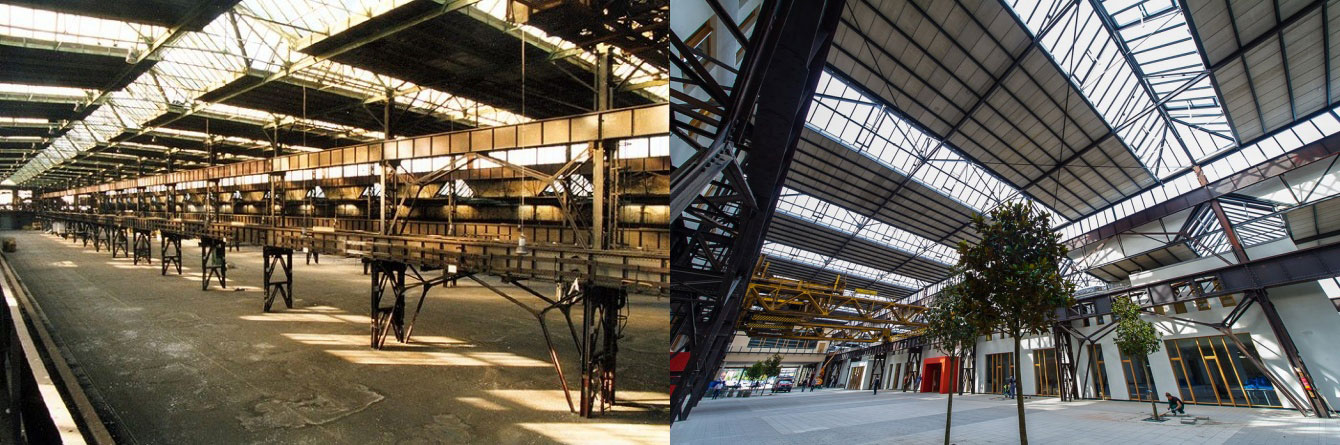
\includegraphics[width=1.0\textwidth]{CampusVorherNachher.jpg}
\caption[Vorher-Nachher-Vergleich]{Der Campus vor (links) und nach dem Umbau (rechts)\protect\footnotemark}
\label{fig:CampusVorher}
\end{figure}
\footnotetext{Bildquellen:\url{http://www.lingen.de/leben_und_wohnen/stadtentwicklung/projekte_staedtebau/campus_lingen/architektur.html}}
